% ID: SEL-D0014-BA-E01
% ESTADO: validada. S015; tres pasadas del mismo autor, sin segundo revisor.
\textbf{Modelo de preparación e ingresos.}\par\nopagebreak[4]
Sean $x$ e $y$ las bolsas del primer y segundo tipo. Las existencias imponen
\[
\begin{cases}2x+y\leq120&\text{(bocadillos)},\\x+y\leq70&\text{(refrescos)},\\x+2y\leq110&\text{(fruta)},\\x\geq0,\quad y\geq0.\end{cases}
\qquad\max F=6x+5y.
\]
En el contexto se cuentan bolsas completas, por lo que $x,y$ son enteros. El óptimo continuo que hallaremos ya cumple esa condición.

\textbf{Recinto y vértices.}\par\nopagebreak[4]
Al intersecar los semiplanos, los vértices factibles, en orden, son
\[
\boxed{(0,0),\ (60,0),\ (50,20),\ (30,40),\ (0,55).}
\]
Los interiores al primer cuadrante salen de las fronteras bocadillos/refrescos y refrescos/fruta. La intersección de bocadillos/fruta, $(130/3,100/3)$, se descarta porque supera los $70$ refrescos.
\begin{center}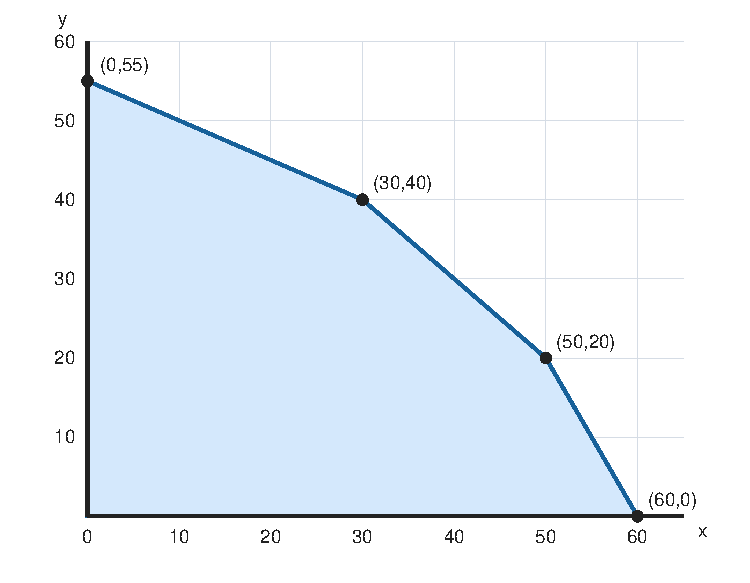
\includegraphics[width=0.56\linewidth]{recursos/figuras/s015-region.pdf}\end{center}
En los vértices, los ingresos son, respectivamente, $0$, $360$, $400$, $380$ y $275$ euros. Por linealidad sobre un polígono compacto,
\[
\boxed{x=50,\quad y=20,\quad F_{\max}=400\text{ euros}.}
\]
Comprobación global: $F=(2x+y)+4(x+y)\leq120+4\cdot70=400$. La igualdad exige ambas fronteras y determina de forma única $(50,20)$. Se consumen $120$ bocadillos, $70$ refrescos y $90$ piezas de fruta.

\textbf{Las otras dos preguntas.}\par\nopagebreak[4]
No se pueden vender $40$ bolsas de cada tipo: necesitarían $80$ refrescos y $120$ frutas, superiores a $70$ y $110$, aunque los $120$ bocadillos sí bastasen. Tampoco pueden obtenerse $410$ euros: exceden la cota máxima demostrada de $400$ euros.
